\documentclass[12pt,a4paper,notitlepage]{article}

\usepackage{./styles/att-1990}

\addbibresource{att-1990.bib}

\newcommand*{\att}{AT\&T}
\newcommand*{\foottitle}{\att{} 1990 Long Distance Network Crash}

\title{
	\vspace{-2\baselineskip}
	
\includegraphics[scale=0.15]{feuplogo.jpg}\\
	{\Huge \att{} 1990 Long Distance Network Crash}\\
	{\Large Overview, Analysis and Consequences}\\
	{\normalsize Software Engineering 2018}
}

\author{
	Bruno Carvalho \hspace*{1em} \text{up201606517}
}

\begin{document}
\maketitle
\thispagestyle{empty}

\subsection{Overview}

The infamous \att{} long-distance telephone network collapse started at 2:25pm on Monday, January 15th 1990, and lasted for about nine hours until engineers managed to patch and stabilize the system.\supercite{att-dennisburke1995}
Approximately half of all calls placed on the network failed to go through, returning a \emph{busy} signal to the caller.

\att{} lost more than \$60 million in unconnected calls, not to mention the amount of revenue lost by businesses heavily reliant on the telephone network, such as airline reservation systems, hotels and delivery companies. Furthermore, this came to have a huge negative impact on the company's reputation, as the network had been extensively advertised as the \textsl{epitome of reliability}.\supercite{att-popularscience1990}

\subsubsection{Long Distance Network Operational Model}

Let's go back to 1990 to see how the network functioned \textsl{on a good day}.

\att{}'s long distance, countrywide telephone network was built on the backbone of a system comprised of 114 computer-operated electronic \emph{switches}, called 4ESS, scattered throughout the US -- each capable of directing about 700.000 calls per hour.

Parallel to this network of switches there were 14 \emph{long-distance routes} capable of holding and transmitting the actual phone calls.\supercite{att-dennisburke1995}

Whenever a call was issued, the phone's local network looked for the receiver's location.
When out of reach it requested the wide network a long range transmission, and the call was delegated up to one of the \emph{switches}, which then scanned all the long-distance routes to establish the connection.
Simultaneously, it sent the receiver's telephone number through a parallel signaling network, which checked for alternate routes involving other minor networks, and, in particular, determined if the receiver's local network could handle the call -- meaning it could be delegated down.

If the network found that the destination switch along the chosen long-distance route was busy, and it also couldn't delegate the call to a local network, it returned to the caller a \emph{busy} signal, releasing the line.
However, if the destination switch signaled available, a reservation was made and a connection was established. The entire process took no longer than $4-6$ seconds,\supercite{att-dennisburke1995} and allowed for real-time communications from coast to coast.

\subsection{Analysis: January 15th Incident}

It all started on the New York switch, which performed a routine self-test and found it was nearing its load limits.
Following procedure, the switch, which we will call $A$, sent a message -- a \textit{congestion signal} -- over the network indicating it would not take any more requests until further notice, and promptly performed a four second reset.

The problem arose when $A$ came back online.
Prior to a recent software update -- aimed at speeding up switch intercommunications -- $A$ would send a message through the network indicating it was back online and ready to receive and send new traffic -- a \textit{revival signal}.
After a very short delay, it would start sending out said traffic.
However, with the recent software update, there were no revival signals anymore, and $A$ proceeded to send traffic immediately.
Another switch, say $B$, would learn that $A$ was back online only when traffic from $A$ reappeared on the network.\supercite{att-risksdigest}

\begin{wrapfigure}[25]{r}[2.5em]{0.4\textwidth}
	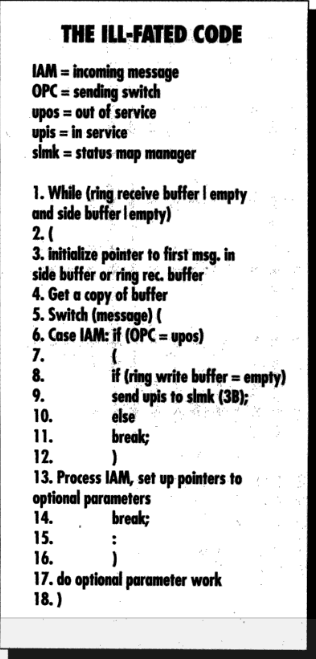
\includegraphics[scale=0.55]{ill-fated-code.jpg}
\end{wrapfigure}

From the perspective of switch $B$, learning that $A$ was back online required it to update some internal records -- presumably the same way as before the software update.

However, recall that $A$ was under stress, and nearing its maximum throughput of about one call every five milliseconds.
The situation was better after the reset (as some traffic had been redirected to other switches) but not by much, so it was still sending traffic to the network at unparalleled speed.
For switch $B$, this implied that the first message it received from $A$, causing it to update its records, was quickly followed by a second message again from $A$, something which did not happen before the update.
This set the precedent for a software bug, which had gone unnoticed in testing, to start wrecking havoc in the system.

\subsubsection{The smallest bug breaks the network}

The defect was found in a \textsf{C} program which contained a misplaced \textit{break} statement (line 11).\supercite{att-dennisburke1995,att-popularscience1990}
The piece of pseudo code shown is invoked whenever a switch receives a message.\supercite{att-popularscience1990}
For $B$, updating its internal records amounts in part to lines 8 and 9 in the code -- writing to the \textsl{ring write buffer}, which behaves like a one-slot message queue to another subsystem in the same switch.

When $B$ got the second message, \textbf{the buffer had not been cleared yet}, so the program would proceed into the else clause and break out of the switch case.
But this meant that line 13, to be run unconditionally, \textbf{was not executed}.
This had severe implications further down the function, namely overwriting the non-empty ring write buffer.

Parallel error correction software would detect this overwrite instantly, and would follow established protocol and shut down switch $B$, resetting it in a fashion similar to that of switch $A$.
And so $A$'s four second intentional reset became $B$'s four second \emph{unintentional} reset.
This cascaded throughout the network, endlessly for nine hours.

Overwriting the ring write buffer is a type of race condition.
Consider all possible switches $B$ -- some would overwrite the buffer, and thus reset, and some would not.
This is what allowed the network to not become completely engulfed in reset madness, and still manage to allow about half of all calls placed on it go through.

\subsection{Lessons Learned}

``Unsurprisingly, it is not difficult for a simple software error to remain undetected, to later bring down even the most reliable systems.''\supercite{att-dennisburke1995}

When we think of high-impact, vast-reaching software bugs, we don't tend to think they could be something as simple as this.

But we know for a fact software is extremely fragile -- and, paradoxically, usually quite strict as well, due to the programming languages used.
Language strictness prevents common mistakes such as unintended type conversions and errors.
Detecting incorrect control flow, however, is the job of an independent tool, specifically a coverage analysis tool.
But still the error would surpass the tool's scrutiny -- which would show unconditional coverage of line 13, as intended -- unless a clever test routine that stressed the switch managed to trigger the race condition.

A more structured programming language would have made this particular defect more likely to pop up at compile time, as the compiler might have detected the race condition, or even impossible to construct.
But perhaps the biggest contributor to this catastrophic failure was the routine practice of resetting switches -- it would be far better if minor problems could be handled without shutting down an entire switch.

It is this tremendous lack of certainty that plagues software engineering in general.
There is no combination of language, tools and testing practices that can guarantee a large software project such as this has no \textsl{errors}, not even inconsequential ones.
It is up to the developers themselves to follow best practices when they write code and establish guidelines, when they design protocols and platforms, and ultimately when they must confront and repair the errors found in their creations.

\printbibliography

\end{document}